\documentclass[11 pt]{scrartcl}
\usepackage[header, margin, koma]{tyler}

\newcommand{\hwtitle}{Calculus and Probability Review}

\pagestyle{fancy}
\fancyhf{}
\fancyhead[l]{\hwtitle{}}
\fancyhead[r]{CS 70 Staff}
\cfoot{\thepage}

% TODO: add a joint pdf example to the double int. section

\begin{document} 
\title{\Large \hwtitle{}}
\author{\large CS 70 Staff}
\date{\large\today}

\maketitle 

This is a quick refresher of single and multi variable calculus in the context of probability. If any material needs refreshing, \cite{stewart} is the canonical calculus textbook, while Khan Academy has fantastic video explanations. Finally, this is a reminder that \textbf{calculus will not be over-emphasized on the final}; after all, this is a probability course, not a calculus course.  
%\tableofcontents

\section{Derivatives}
Single variable calculus starts with the notion of a derivative, which represents the \emph{instantaneous} rate of change of a function $f(x)$. Formally, 

\begin{definition}[Derivative]
    The \textbf{derivative} of a function $f(x)$ is defined to be
    \[ f'(x) = \lim_{h\to 0} \dfrac{f(x+h)-f(x)}{h}.\]
    We sometimes also denote it by $\frac{df}{dx}$ or $\frac{d}{dx} f(x)$ to emphasize that the derivative is with respect to $x$. 
\end{definition}

The idea is that this value gives us the slope of the secant line passing through $(x, f(x))$ and $(x+h, f(x+h))$, and as $h$ becomes smaller and smaller, the secant line becomes the tangent line at the point $x$. 

This definition is seldomly used once we know the basics of dealing with derivatives though. That comes in the form of the following common forms and properties. Assume $c\in \RR$ is a constant. 

\begin{itemize}
    \ii $\frac{d}{dx} c = 0$.
    \ii $\frac{d}{dx} x^n = nx^{n-1}$. 
    \ii $\frac{d}{dx} \sin x = \cos x$.
    \ii $\frac{d}{dx} \cos x = -\sin x$.
    \ii $\frac{d}{dx} e^x = e^x$ (the only such function!).
    \ii $\frac{d}{dx} c^x = c^x\ln c$.
    \ii $\frac{d}{dx} \ln x = \frac{1}{x}$.
\end{itemize}

Of course, derivatives add and subtract, and with the next two rules, you're ready to differentiate nearly any function you come across. 

\begin{lemma}[Product Rule]
    For any two functions $f(x)$ and $g(x)$,
    \[ \dfrac{d}{dx} (f\cdot g)(x) = f'(x) g(x) + f(x)g'(x) \] 
    or in other words, 
    \[ (fg)' = f'g + fg'.\]
\end{lemma}

\begin{lemma}[Chain Rule]
    Suppose I have a function $f(x) = g(h(x))$. Then 
    \[ f'(x) = g'(h(x))\cdot h'(x).\] 
    Equivalently, 
    \[ \dfrac{df}{dx} = \dfrac{df}{dh} \dfrac{dh}{dx}.\] 
\end{lemma}

In other words, I keep unrolling my derivatives from outside in when I use the chain rule. 

\begin{example}
    Compute the derivative of $f(x) = x^2e^{2x}$.  
\end{example}
\begin{proof}[Solution]
    Applying the product rule followed by the chain rule gives 
    \[ f'(x) = (x^2)'e^{2x} + x^2 (e^{2x})' = 2xe^{2x} + x^2 e^{2x} (2x)' = 2xe^{2x} + 2x^2e^{2x}.\] 
\end{proof}

\begin{exercise}
    Find the derivatives of the following functions: 
    \alphanum
        \ii $F(x) = 5(5-x)^4$
        \ii $F(x) = e^{-3x}$
        \ii $F(x) = \sqrt{x^3}$
    \enumend
\end{exercise}

\section{Integrals}
\subsection{Definitions}
Complementing the derivative is first the \emph{definite} integral, which represents the signed\footnote{Meaning positive if we're above the $x$-axis and negative otherwise.} area under the curve. The nice interpretations and motivations for this come from physics, so I'll move on and give an informal definition. 

\begin{definition}[Definite Integral]
    The \textbf{definite integral} $\int_a^b f(x) dx$ is the signed area of the region of the $xy$-plane bounded by the graph of $f$, the $x$-axis, and the vertical lines $x = a$, $x = b$.   
\end{definition}

\begin{figure}[!htb]
    \centering
    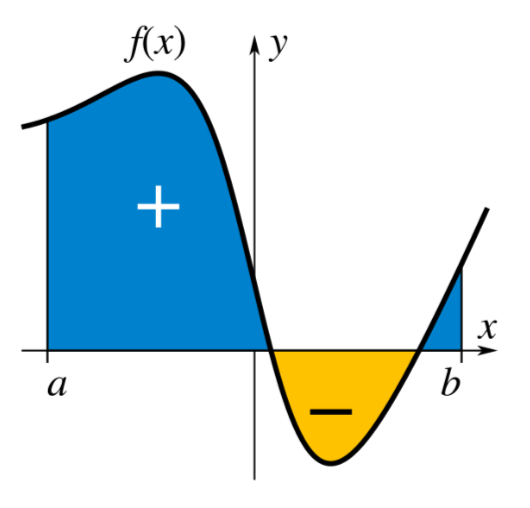
\includegraphics[scale=0.5]{def_integral.png}
    \caption{An example of such an integral.}
\end{figure}

It turns out that integration and differentiation are inverse operations. So we have the notion of an \emph{antiderivative}, a function $F$ whose derivative is a given function $f$, which is also sometimes called an \emph{indefinite} integral. 

\begin{definition}[Indefinite Integral]
    An antiderivative $F(x)$ of $f(x)$ is called an \textbf{indefinite integral}, and written as 
    \[ F(x) =  \int f(x) dx.\] 
\end{definition}

One important point to note is that since constants vanish under differentiation, given an antiderivative $F(x)$, any other function $F(x) + c$ where $c$ is a constant is also an antiderivative. Never forget to plus $c$! 

In the midst of all this back and forth, it's still not clear at all how we'd compute the area under the curve in order to actually find the definite integral. This is where the Fundamental Theorem of Calculus comes into play; it creates the connection between the definite and indefinite integrals (and therefore between definite integrals and derivatives). 

\begin{theorem}[Fundamental Theorem of Calculus]
    If $f$ is a real-valued, integrable function on $[a,b]$, and $F$ is an antiderivative of $f$ on $[a,b]$ (so that $F' = f$), then 
    \[ \int_a^b f(x) dx = F(b) - F(a).\] 
\end{theorem}

This theorem is paramount for going back and forth between integrals and derivatives. If you think about it, this theorem is what lets us use CDFs to evaluate our pdfs. So under the surface, problems like Example~\ref{example:ft_rv} are really using the fundamental theorem somewhere. 


Here are some common integrals you should know: 
\begin{itemize}
    \ii $\int x^n\; dx = \frac{x^{n+1}}{n+1} + C$ for $n \not= -1$. 
    \ii $\int \frac{1}{x}\; dx = \ln |x| + C$
    \ii $\int e^x\; dx = e^x + C$ 
    \ii $\int \sin x\; dx = - \cos x + C$
    \ii $\int \cos x\; dx = \sin x + C$
\end{itemize}

\begin{example}
    Compute $\int_0^4 x^2 dx$. 
\end{example}
\begin{proof}[Solution]
    By inspection (or by looking at the list above) we find that an antiderivative is $F(x) = \frac{x^3}{3}$, and so by the fundamental theorem, our answer is just $F(4) - F(0)$. Written more concisely, 
    \[ \int_0^4 x^2 dx = \dfrac{x^3}{3}\Big\rvert^4_0 = \dfrac{4^3}{3} - \dfrac{0}{3} = \dfrac{64}{3}.\] 
\end{proof}

\subsection{Integrating techniques: $u$-sub, integration by parts, and others}
There's two common techniques you'll use when solving integrals. The first is pretty simple. It's utilizing a change of variables, otherwise known as $u$-substitution. 

\begin{example}
    Compute $\int_0^5 e^{-6x}dx$. 
\end{example}
\begin{proof}[Solution]
    This isn't an integral of one of the above forms since we have extra coefficients in the exponent, so we'll perform a change of variables to get it to look like it. Let $u = -6x$, so $du = -6 dx$ or $-\frac 16 du = dx$. Now if we change variables, we will get an antiderivative of 
    \[\int e^{-6x} dx = \int -\frac 16 e^{u} du = -\frac 16 e^u + C = -\frac 16 e^{-6x} + C.\] 
    
    Plugging this in gives 
\[ \int_0^5 e^{-6x} dx = -\frac 16 e^{-6x} \Big\rvert^5_0 = -\frac 16 e^{-30} + \frac 16 .\]
\end{proof}

The second technique is \emph{integration by parts}, which is not as straightforward. The idea is that we want to be able to integrate products of functions that aren't as nice. This reminds us of the product rule for derivatives, which states that if I had two functions $u(x)$ and $v(x)$, then 
\[ (uv)' = u'v + uv'.\] 

Integrating both sides with respect to $x$ gives 
\[ u(x) v(x) = \int (u(x) v(x))' dx  = \int u'(x) v(x) dx + \int u(x) v'(x) dx \]

If we use differentials and let $du = u'(x) dx$ and $dv = v'(x) dx$,\footnote{A differential is change in the function based on the dependent variable (how far up we move based on horizontal movement and the slope).} we can write this in a format thats more recognizable, namely 
\[ u(x) v(x) = \int v(x) du + \int u(x) dv \implies \boxed{\int u\; dv = uv - \int v\; du}.\] 

So now we can take an integral that's hard to compute, and flip around what we're integrating to make it potentially easier to simplify. It's easiest to understand through an example. 

\begin{example}
    Compute $\int xe^{3x}\; dx$. 
\end{example}
\begin{proof}[Solution]
    If I'm applying integration by parts, I need to find one expression to take the derivative of (which will be $u$) and another to take the integral of (which will be $dv$) to simplify. Here, I'll let $u = x$ and $dv = e^{3x} dx$, so that $du = dx$ and $v = \frac 13 e^{3x}$. Then applying integration by parts gives 
    \[ \int xe^{3x} = \int u\; dv = uv - \int v\; du = \frac 13 xe^{3x} - \int \frac 13 e^{3x} dx = \frac 13 xe^{3x} - \frac 19 e^{3x} + C.\] 
\end{proof}

It's not always obvious what I should be setting $u$ and $dv$ to typically. A good rule of thumb is to set $u$ to the first term you see in this list: 
\begin{itemize}
    \ii Logarithm 
    \ii Inverse trig function 
    \ii Algebraic function (e.x. polynomials)
    \ii Trig function 
    \ii Exponential function
\end{itemize}

Here's another example. 
\begin{example}
    Compute $\int \ln x \; dx$.  
\end{example}
\begin{proof}[Solution]
    You might think that we can't apply integration by parts here since we only have one term. But in fact, let $u = \ln x$ and $dv = dx$ so that $du = \frac{1}{x} dx$ and $v = x$. Then 
    \[ \int \ln x\; dx = \int u \; dv = uv - \int v\; du = x\ln x - \int x\cdot \frac{1}{x} \; dx = x\ln x - x + C.\] 
\end{proof}

You should also search for the tabular method if you want to speed things up when doing multiple integrations by parts (Khan academy is a good place to watch). 

\begin{exercise}
    Compute $\int x^2e^{3x}\; dx$. 
\end{exercise}

\section{Series}
A quick informal definition so everyone's on the same page here. 

\begin{definition}[Series]
    Given some sequence of terms $(a_1, a_2, \dots, a_n)$, the \textbf{series} corresponding to this sequence is the sum 
    \[ a_1 + a_2 + \dots + a_n.\] 
    If the sequence is infinite, then the series will contain infinitely many summands. 
\end{definition}

Series come up often in discrete probability when we ask what the probability of some range of events is. So it's useful to know how to sum the two main types of series and some tricks we can do with them. 

There's two main series to know: the geometric series, and the Taylor series.

In a geometric series, we have an initial term $a$, and every term after that is some common ratio, $r$, times the previous terms. So a typical finite geometric series looks something like 

\[ S = a + ar + ar^2 + \dots + ar^k\] 

where $S$ is the final value of the series. To calculate this, notice that 

\[ rS = ar + ar^2 + \dots + ar^k + ar^{k+1},\] 

so if we subtract one from the other, all the middle terms cancel out, leaving us with 

\[ S - rS = a - ar^{k+1} \implies \boxed{S = \dfrac{a(1-r^{k+1})}{1-r}}.\] 


If we take $k \to \infty$, then we get an infinite geometric series, for which 
\[ \sum_{i=0}^\infty ar^i = \dfrac{a}{1-r}\] 

but only when $|r| < 1$ (otherwise the series won't converge). Here's an example that utilizes geometric series for a very fitting distribution.
\begin{example}
    Show that the sum of the probabilities of a random variable $X \sim \Geo(p)$ is 1. 
\end{example}
\begin{proof}[Solution]
    Recall that $\PP(X = k) = (1-p)^{k-1} p$. Then 
    \[ \sum_{k=1}^\infty \PP(X=k) = \sum_{k=1}^\infty (1-p)^{k-1} p.\] 
    But this is a \emph{geometric} series with initial term $p$ and ratio $1-p$, so the sum is $\frac{p}{1-(1-p)} = 1$. 
\end{proof}

The idea of a Taylor series is to approximate a function $f(x)$ by its derivatives. This looks like 

\[ f(x) = f(0) + f'(0)x + \dfrac{1}{2!} f''(0) x^2 + \dfrac{1}{3!} f'''(0)x^3 + \dots = \sum_{k=0}^\infty \dfrac{1}{k!}f^{(k)}(0)x^k\] 

where $f^{(k)}$ is the $k$th derivative of $f$. The only one you'll need for this class is $e^x$: 

\[ e^x = 1 + x + \dfrac{x^2}{2!} + \dfrac{x^3}{3!} + \dots = \sum_{k=0}^\infty \dfrac{x^k}{k!}.\] 

One last interesting note is that geometric series are \emph{also} Taylor series. If we let $f(r) = \frac{a}{1-r}$, then the derivatives are 

\[ f(r) = \frac{a}{1-r}, \quad\quad f'(r) = \frac{a}{(1-r)^2}, \quad\quad f''(r) = 2!\cdot\frac{a}{(1-r)^3}, \quad\dots,\quad f^{(k)}(r) = k!\cdot \dfrac{a}{(1-r)^{k+1}} \]

so 

\[ f(0) = a, \quad\quad f'(0) = 1!\cdot a, \quad\quad f''(0) = 2!\cdot a, \quad\dots,\quad f^{(k)}(0) = k!\cdot a.\]

Plugging this into the Taylor series expansion gives 

\[ f(r) = \dfrac{a}{1-r} = a + ar + ar^2 + \dots\]

which is the geometric distribution as expected. 

\begin{exercise}
    Show that the sum of the probabilities of a Poisson random variable $X\sim \text{Poisson}(\lambda)$ is 1. 
\end{exercise}

\section{Intermission: Calculus and Series in Probability}
Now that we've covered some calculus, let's look at how the different results we've seen so far are used in probability. 

Here's two problems that make use of the Taylor series for $e^x$. 
\begin{example}[Dis 12 \#3]
    Let $X \sim \Geo(p)$ and $Y \sim \Poisson(\lambda)$ be independent random variables. Compute $\PP(X > Y)$. 
\end{example}
\begin{proof}[Solution]
    Let's condition on $Y$ so that we can use $\PP(X > k) = (1-p)^k$. This gives 
    \begin{align*}
        \PP(X > Y) &= \sum_{y=0}^\infty \PP(Y=y) \PP(X > y | Y = y) \\ 
                   &= \sum_{y=0}^\infty \dfrac{e^{-\la}\la^y}{y!}\cdot (1-p)^y \\ 
                   &= e^{-\la}\sum_{y=0}^\infty \dfrac{(\la(1-p))^y}{y!} 
    \end{align*}
    But this sum is the Taylor series for $e^{\la(1-p)}$, so the probability is just $e^{-\la}e^{\la-\la p} = e^{-\la p}$. 
\end{proof}

This somewhat surprising result was derived in Lecture 21. 
\begin{example}
    Let $X_n$ be a random variable counting the number of fixed points of a permutation on $n$ variables. What is the distribution of $X_n$ as $n\to\infty$?  
\end{example}
\begin{proof}[Solution]
    We wish to compute $\PP(X_n = j)$, so we count the number of permutations with $j$ fixed points. We need to choose $j$ points to be fixed and the rest to not have any fixed points, which means they form a derangment, so there are $\binom{n}{j}D_{n-j}$ such permutations. Hence 
    \[ \PP(X_n = j) = \dfrac{\binom{n}{j}  D_{n-j}}{n!}.\]

    Recalling that $D_j = j!\sum_{k=0}^j \frac{(-1)^k}{k!}$, we find 
    \begin{align*}
        \PP(X_n = j) &= \dfrac{1}{n!}\left[ \dfrac{n!}{j!(n-j)!} (n-j)! \sum_{k=0}^{n-j}\dfrac{(-1)^k}{k!}\right] \\ 
                     &= \dfrac{1}{j!} \sum_{k=0}^{n-j}\dfrac{(-1)^k}{k!}.
    \end{align*}
    But when $n\to\infty$, this is the Taylor Series for $e^{-1}$, so 
    \[ \lim_{n\to\infty} \PP(X_n = j) = \frac{e^{-1} 1^j }{j!} \] 
    which is the pdf of a $\Poisson(1)$ distribution. 
\end{proof}
This result also agrees with the fact that $\EE[X_n] = 1$, which is true by linearity of expectation.  

Here's an idea similar to Discussion 13, Problem 2 but in a different context. Under the hood, you should realize that we can do this cdf manipulation thanks to the Fundamental Theorem of Calculus. 
\begin{example}
    Let $X, Y$ be a random variables where $Y = X^2$. Express the pdf of $Y$, $f_Y$, in terms of the pdf of $X$, $f_X$.   
    \label{example:ft_rv}
\end{example}
\begin{proof}[Solution]
    The first step should usually be to compute the cdf of $Y$ in terms of $X$'s cdf. This gives 
    \[ F_Y(x) = \PP(Y \leq x) = \PP(X^2 \leq x) = \PP(-\sqrt{x} \leq X \leq \sqrt{x}) = F_X(\sqrt{x}) - F_X(-\sqrt{x}).\] 
    From here, we differentiate with respect to $X$ (being careful to use the chain rule) and get 
    \[ f_Y(x) = \dfrac{dF_Y}{dx} = \dfrac{1}{2\sqrt{x}}F_X'(\sqrt{x}) - \left(-\dfrac{1}{2\sqrt{x}}\right)F_X'(-\sqrt{x}) 
    = \dfrac{1}{2\sqrt{x}} (f_X(\sqrt{x})+f_X(-\sqrt{x})) \]

\end{proof}

\section{Double Integrals}
Now we're finally talking about multivariable calculus. Before we start, we should ask the question: what even is a double integral? 

We should first think about what a single integral represented. In summary, we defined it as 
\[ \boxed{\text{Finding an \textcolor{blue}{area} under } f(x) \text{ over a \textcolor{blue}{one-dim. interval} } {\color{blue} [a,b]} \text{ on the } {\color{blue} x \text{-axis: }} A = \int_a^b f(x) \; dx.}\] 

The double integral will be the natural generalization of this. Instead of integrating an area over an interval, we will be integrating a volume over a region in 2D space. 
\[ \boxed{\text{Finding a \textcolor{red}{volume} under } f(x,y) \text{ over a \textcolor{red}{two-dim. region} } {\color{red} \mathcal{R}} \text{ on the } {\color{red} xy \text{-plane: }} V = \iint_\mathcal{R} f(x,y) \; dA.}\] 

The hardest part of solving double integrals is often figuring out the region of integration and setting up the limits. After that, it's just single-variable calculus. Let's look at an example. 

\begin{example}
    Integrate $f(x,y) = x^2 + y^2$ over the $4\times 4$ square centered at $(0,0)$. 
\end{example}
\begin{proof}[Solution]
Before we begin, take a look at this visualization of our integral. 

\begin{figure}[!htb]
    \centering
    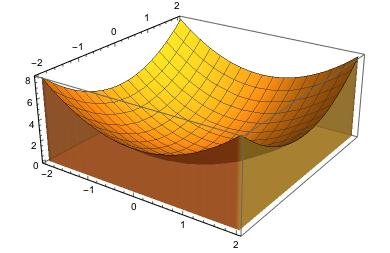
\includegraphics[scale=0.5]{x2y2.jpeg}
    \caption{A visualization of the integral of $f(x,y) = x^2 + y^2$ over the square $[-2,2]\times [-2,2]$.}
\end{figure}

As you can tell, we're looking for the volume under the curve. Our region of integration is the region bounded by the lines $x = -2, x = 2, y = -2, y = 2$. 

There's two ways in which we can integrate over this region: we can either integrate with respect to $x$ first, or with respect to $y$ first. Either way is the same in this case since everything is symmetric, so I'll set it up as the former. 
    This means our integral is 
\[ \int_{-2}^2 \int_{-2}^2 x^2+y^2 \; dx \; dy.\]

In order to integrate this, we treat the inside integral like a single integral and treat everything that's not $x$ like a constant. This gives 

\[ \int_{-2}^2 \int_{-2}^2 x^2+y^2 \; dx \; dy = \int_{-2}^2 \left(\frac{x^3}{3}+xy^2\right)\Big\rvert^2_{x=-2} \; dy = \int_{-2}^2 \frac{16}{3} + 4y^2 \; dy\]

Now that we've gotten rid of our $x$ variable (as expected), all that's left is to finish the single integral, which gives us 

\[ \int_{-2}^2 \frac{16}{3} + 4y^2 \; dy = \left(\frac{16}{3}y + \frac{4}{3} y^3\right)\Big\rvert^{2}_{-2} = \frac{128}{3}.\]
\end{proof}

Here's one where the region of integration is trickier. 

\begin{example}
    Integrate $ye^{-x}$ over the \emph{triangle} enclosed by $y = x$, $y = 3$, and $x = 0$. 
    \label{ex:ye-x}
\end{example}
\begin{proof}[Solution]
    \begin{figure}[!htb]
        \centering
        \begin{minipage}{0.45\linewidth}
            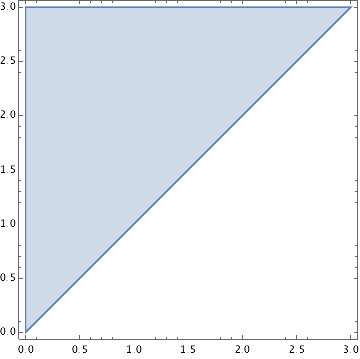
\includegraphics[scale=0.35]{boundary.png}
        \end{minipage}%
        \begin{minipage}{0.45\linewidth}
            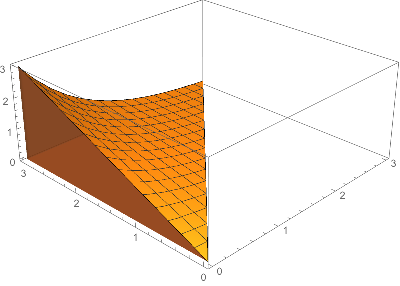
\includegraphics[scale=0.45]{ye-x.png}
        \end{minipage}%
        \caption{The boundary and the integral of $f(x,y) = ye^{-x}$ over the region in Example~\ref{ex:ye-x}.}
    \end{figure}

    We already know the region is a triangle, but we need to figure out how to integrate over it. If we first integrate over $y$ then $x$, then the limits of our outer integral should go from $0$ to 3. In this case, we then have the variable $x$ to work with to set up our limits for $y$. Using the equations, we find that we should integrate from $x$ to $3$. Setting up our integral and simplifying gives 

    \begin{align*}
    \int_0^3 \int_x^3 ye^{-x} \; dy \; dx &= \int_0^3 \frac 12 (y^2 e^{-x})\Big\rvert^3_{y = x} \; dx \\ 
                                          &= \frac 12 \int_0^3 9e^{-x} - x^2e^{-x}\; dx
    \end{align*}
    
    which would require the use of \emph{two} integrations by parts to evaluate; yuck! Let's see what happens if we set up our integral the other way. The outer limits are still from 0 to 3, but the inner ones are now from 0 to $y$ (convince yourself of this), so the integral is 
    \begin{align*}
    \int_0^3 \int_0^y ye^{-x} \; dx \; dy &= \int_0^3  (-y e^{-x})\Big\rvert^y_{x = 0} \; dy  = \int_0^3 -y e^{-y} + y \; dy \\ 
                                          &= \int_0^3 y \; dy - \left(-ye^{-y}\Big\rvert^3_0 + \int_0^3 e^{-y}\; dy \right) \\ 
                                          &= \frac{9}{2} - (-3e^{-3} + 1 - e^{-3}) = \boxed{\frac{7}{2} + \frac{4}{e^3}}.
    \end{align*}
\end{proof}

We don't always have to integrate using $x$ and $y$ though. Sometimes it's more natural for us to use \emph{polar} coordinates where we label every point as $(r, \theta)$, $r$ being its distance from the origin and $\theta$ being its angle with the $x$-axis. 

\begin{example}
    Integrate $f(x,y) = x^2 + y^2$ over the circle of radius $2$ centered at $(0,0)$. 
\end{example}
\begin{proof}[Solution]
    The first step is to translate our function in terms of $r$ and $\theta$. We know that $x^2 + y^2 = r^2$, so $f(r, \theta) = r^2$. Our region is $0\leq r \leq 2$, so our integral is 

\[ \int_{0}^{2\pi} \int_{0}^2 r^2 \; dr\; d\theta = \int_0^{2\pi} \frac{r^3}{3} \Big\rvert^2_{r=0} \; d\theta = \int_0^{2\pi} \frac{8}{3} \; d\theta = \dfrac{16}{3}\pi.\] 
\end{proof}
We did something similar with Buffon's needle, where we integrated with respect to $y$ and $\theta$. All that matters is that we find the appropriate regions and limits to integrate over. 

\begin{exercise}
    Integrate $e^{x+y}$ over the rectangular region determined by the lines $y = 0$, $x = 0$, $y = 3$, $x = 2$. 
\end{exercise}
\begin{exercise}
    Integrate $-\frac{xe^x}{y^2}$ over the region defined by the lines $x = 5$, $y = -x$, $y = x$. 
\end{exercise} 
\begin{exercise}
    Suppose $X \sim \Exp(\la_1), Y \sim \Exp(\la_2)$ are independent exponential distributions so that $f(x,y) = \la_1\la_2 e^{-(\la_1+\la_2)x}$ for $x, y \geq 0$ is the density of their joint distribution. 
    Show that the integral of this density is 1. % over its support.\footnote{The \emph{support} a function $f$ are all inputs where its nonzero. For example, the support of a uniform random variable on $[a,b]$ is just $[a,b]$.}
\end{exercise}

%\section{Joint Densities of Continuous Random Variables}


\begin{thebibliography}{12}
	\bibitem{stewart}
		James Stewart, \textit{Calculus 7 ed}. Cengage Learning, 2012. 
\end{thebibliography}





\end{document}
